
\chapter{Iteración}
\label{iteration}

Este capítulo es sobre iteración, la cual es la habilidad
para ejecutar un bloque de sentencias repetidamente. Vimos
un tipo de iteración, usando recursión, en la Sección~\ref{recursion}.
También vimos otro tipo, usando un bucle {\tt for}, en la
Sección~\ref{for_loops}. En este capítulo veremos otro tipo, 
usando la sentencia {\tt while}. Pero primero queremos discutir
un poco más sobre la asignación de variable.

\section{Asignación Versus Igualdad}
\index{assignment!operator}
\index{equality operator}

Antes de proceder, quiero hablar sobre una fuente común de confusión.
Dado que Perl usa el signo de igualdad ({\tt =}) para la asignación, 
es tentativo interpretar una sentencia como {\tt \$a = \$b} como 
una proposición matemática de igualdad, eso es, la afirmación que 
{\tt \$a} y {\tt \$b} son iguales. Pero esta interpretación es incorrecta.
\index{equality and assignment}

Primero, la igualdad es una relación simétrica y la asignación no lo es. 
Por ejemplo, en matemática, si $a = 7$, entonces $7 = a$. Pero en Perl, 
la sentencia {\tt \$a = 7} es legal y {\tt 7 = \$a} no lo es.

De igual manera, en matemática, un proposición de igualdad es verdadera
o falsa todo el tiempo. Si $a = b$ ahora, entonces $a$ siempre será igual
a $b$. En Perl, una sentencia de asignación puede hacer dos variables iguales,
pero no tienen que permanecer de ese modo:

\begin{verbatim}
> my $a = 5;
5
> my $b = $a;   # $a y $b son iguales ahora
5
> $a = 3;       # $a y $b ya no son iguales
3
> say $b;
5
\end{verbatim}
%
La tercera línea cambia el valor de {\tt \$a} pero no cambia el 
valor de {\tt \$b}, así que ya no son iguales.

En resumen, recuerda que {\tt =} es un operador de asignación y
no un operador de igualdad; los operadores para probar igualdad entre
dos términos son {\tt ==} para números y {\tt eq} para cadenas de 
texto.
\section{Reasignación}
\index{assignment}
\index{statement!assignment}
\index{reassignment}

Como tal vez descubriste, es legal hacer más de una asignación a la 
misma variable. Una asignación nueva hace que una variable existente
haga referencia a un nuevo valor (y pare de referirse al valor antiguo):

\begin{verbatim}
> my $x = 5;
5
> say $x;
5
> $x = 7;
7
> say $x
7
\end{verbatim}
%
La primera vez mostramos a {\tt \$x},
su valor es 5; la segunda vez, su valor es 7.

La figura~\ref{fig.assign2} muestra como la {\tt reasignación}
luce en un diagrama de estado. 
\index{state diagram} \index{diagram!state}

Reasignar variables es usualmente útil, pero deberías utilizar esta
característica con cierta precaución. Si los valores de las variables 
se cambian frecuentemente, puede hacer el código difícil de leer y depurar.

\begin{figure}
\centerline
{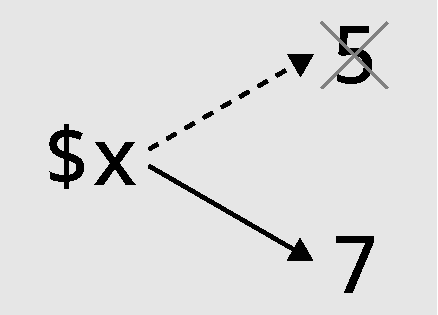
\includegraphics[scale=0.5]{figs/reassignment.pdf}}
\caption{Diagrama de estado.}
\label{fig.assign2}
\end{figure}



\section{Actualización de las Variables}
\label{update}

\index{update}
\index{variable!updating}

Un tipo común de reasignación es una {\bf actualización},
donde el nuevo valor de la variable depende en el viejo:

\begin{verbatim}
> $x = $x + 1;
\end{verbatim}
%
Esto significa ``obtén el valor actual de {\tt \$x}, agrega uno, y después
actualiza {\tt \$x} con el valor nuevo.``

Si intentas actualizar una variable que no se le ha dado un valor,
obtienes una advertencia, porque Perl evalúa el lado derecho de la 
sentencia de asignación antes de que asigne un valor a {\tt \$x}:

\begin{verbatim}
> my $x;
> $x = $x + 1;
Use of uninitialized value of type Any in numeric context 
 in block <unit> at <unknown file> line 1
\end{verbatim}
%
Antes de actualizar una variable, tienes que declararla 
e {\bf inicializarla}, usualmente con una sentencia de asignación:
\index{initialization (before update)}

\begin{verbatim}
> my $x = 0;
> $x = $x + 1;
\end{verbatim}
%
Actualizar una variable al agregar 1 se conoce como un {\bf incremento};
substraer 1 se conoce como un {\bf decremento}.
\index{increment operator}
\index{decrement operator}

Como se mencionó anteriormente en la Sección~\ref{expr_and_statements},
Perl tiene algunos atajos para el incremento y el decremento:

\begin{verbatim}
$x += 1; # equivalente a $x = $x + 1
$x++;    # también equivalente 

$x -= 1; # equivalente a $x = $x - 1
$x--;    # también equivalente 
\end{verbatim}

\section{La Sentencia {\tt while}}
\index{statement!while}
\index{while loop}
\index{loop!while}
\index{iteration}

Las computadoras usualmente automatizan tareas repetitivas.
Repetir tareas idénticas o similares sin hacer errores es algo que las computadoras saben hacer bien y las personas
no tan bien. En un programa de computadora, la repetición se
conoce como {\bf iteración}.

Ya hemos visto dos funciones, {\tt cuenta-regresiva} 
y \verb|imprime-n-veces|, que iteran usando recursión (
ver Sección~\ref{recursion}). Dado que la iteración es tan
común, muchos lenguajes de programación incluyendo a Perl 6
proveen características para hacerla más fácil. Una de ellas es la sentencia {\tt for} que vimos en la Sección~\ref{for_loops}. Regresaremos a eso más tarde.

Otra es la sentencia {\tt while}. Ésta es una versión de 
{\tt cuenta-regresiva} que usa la sentencia {\tt while}:

\begin{verbatim}
sub cuenta-regresiva(Int $n is copy) {
    while $n > 0 {
        say $n;
        $n--;
    }
    say '¡Despegue!';
}
\end{verbatim}
%
Puedes casi leer la sentencia {\tt while} como si fuera inglés.
Significa, ``Mientras (while) {\tt \$n} sea mayor que 0,
muestra el valor de {\tt \$n} y después reduce {\tt \$n}. Cuando 
llegues a 0, muestra la palabra {\tt ¡Despegue!}``
\index{flow of execution}

Aquí se presenta el flujo de ejecución de una sentencia {\tt while}
más formalmente:

\begin{enumerate}

\item Determina si la condición es verdadera o falsa.

\item Si es falsa, abandona la sentencia {\tt while}
y continua la ejecución en la siguiente sentencia.

\item Si la condición es verdadera, ejecuta el cuerpo y
después regresa al paso 1.

\end{enumerate}

Este tipo de flujo se llama un bucle (\emph{loop} en inglés)
porque el tercera paso regresa de nuevo al principio. 
\index{condition}
\index{loop}
\index{body}

El cuerpo del bucle debería cambiar el valor de una o más variables
para que la condición se vuelva falsa eventualmente y el bucle
termine. De lo contrario, el bucle se repetirá por siempre, lo cual 
se llama un {\bf bucle infinito}. Una fuente de entretenimiento para
los científicos de la computación es la observación de que las instrucciones
en la botella de champú, ``Enjabona, enjuage, repite``, son un bucle 
infinito.
\index{infinite loop}
\index{loop!infinite}

En el caso de {\tt cuenta-regresiva}, podemos probar que el bucle
termina: si {\tt \$n} es cero o negativo, el bucle nunca se ejecuta.
Por lo contrario, {\tt \$n} se vuelve más pequeño cada vez a través del
bucle, así que eventualmente tenemos que llegar a 0.

Para otros bucles, no es tan fácil decir si el bucle termina. Por ejemplo:

\begin{verbatim}
sub secuencia($n is copy) {
    while $n != 1 {
        say $n;
        if $n %% 2 {        # $n es par
            $n = $n / 2;
        } else {            # $n es impar
            $n = $n*3 + 1
        }
    }
    return $n;
}
\end{verbatim}
%
La condición de est bucle es {\tt \$n =! 1}, así que el bucle continuará
hasta que {\t \$n} sea {\tt 1}, lo cual hace la condición falsa.

Cada vez a través del bucle, el programa muestra el valor de {\tt \$n}
y después chequea si es par o impar. Si es par, {\tt \$n} es dividido por 2.
Si es impar, el valor de {\tt \$n} es reemplazado con {\tt \$n*3 + 1}. Por ejemplo,
si el argumento que se pasa a {\tt secuencia} es 42, los valores resultantes
de {\tt n} son 42, 21, 64, 32, 16, 8, 4, 2, 1. 

Dado que {\tt \$n} algunas veces incrementa y otras disminuye, no hay prueba
obvia que {\tt \$n} llegará a 1, o que el programa termina. Para algunos valores
particulares de {\tt n}, podemos probar que el programa termina. Por ejemplo, si 
el valor inicial es una potencia de dos, {\tt n} será un par a través del bucle
hasta que llega al 1. El ejemplo anterior termina con tal secuencia de potencias
de dos, comenzando con 64.
\index{Collatz conjecture}

¡La pregunta difícil es si podemos probar que este programa termina para 
{\em todos} los valores positivos de {\tt n}. Hasta ahora, nadie ha sido capaz
de probarlo o refutarlo! (Ver \url{https://es.wikipedia.org/wiki/Conjetura_de_Collatz}.)

Como ejercicio, podrías escribir de nuevo la función 
\verb|imprimir-n-veces| de la Sección~\ref{recursion}
usando iteración en lugar de recursión.

\index{statement modifier}
\index{postfix!syntax}
La sentencia {\tt while} puede también usarse como un modificador de sentencia (o sintaxis sufija):

\begin{verbatim}
my $val = 5;
print "$val " while $val-- > 0;   # imprime 4 3 2 1 0
print "\n";
\end{verbatim}

La sentencia {\tt while} del bucle ejecuta el bloque mientra la 
condición sea verdadera. También existe un bucle {\tt until},
el cual ejecuta el bloque mientra su condición se falsa:
\index{until loop}

\begin{verbatim}
my $val = 1;
until $val > 5 {
    print $val++;                 # imprime 12345
}
print "\n";
\end{verbatim}

\section{Variables Locales y Ámbito de una Variable}

Hemos visto en la Sección~\ref{localvar} que las variables
creadas dentro de una subrutina (con la palabra clave {\tt my}
son \emph{locales} a esa subrutina. La palabra clave {\tt my}
es usualmente llamada un \emph{declarador} porque 
se usa para declarar una variable nueva (o otro identificador).
Es uno de los declaradores más comunes. Ente otros declaradores
se encuentran {\tt our} o {\tt state}, los cuales se describen
brevemente más tarde en este capítulo.
\index{lexical scope}
\index{lexical variable}
\index{variable!lexical}
\index{my}
\index{declarator}

Similarmente, los parámetros de una subrutina son usualmente
\emph{locales} a la subrutina en la signatura donde son
declarados.
\index{subroutine parameters}

Mencionamos brevemente que el término \emph{ámbito lexical}
es probablemente más preciso que local, pero era muy temprano
en ese punto para realmente explicar lo que esto significa.

La declaración de una variable con {\tt my} le da un \emph{ámbito lexical}.
Esto significa que solo existe dentro del bloque actual. En términos
generales, un bloque es una pieza de código de Perl dentro de llaves.
Por ejemplo, el cuerpo de una subrutina y el código de un bucle 
{\tt while} o {\tt for} o de una sentencia condicional {\tt if} 
son bloques de códigos. Cualquier variable creada con el declarador
{\tt my} existe y está disponible solo para usarse dentro del 
lugar donde fue declarada y el final del bloque de código.
\index{bracket!curly}
\index{curly bracket}

Por ejemplo, este código:

\begin{verbatim}
if $condición eq True {
    my $foo = "bar";
    say $foo;  # imprime "bar"
}
say $foo;      # ERROR: "Variable '$foo' is not declared ..."
			   # ERROR: "La variable '$foo' no está declarada ..."
\end{verbatim}
%
fallará en la segunda sentencia de impresión, porque la llamada de la función
\verb|say| no está en el ámbito lexical de la variable {\tt \$foo}, 
el cual termina con llave derecha que cierra el bloque de la condición.
Si queremos que esta variable pueda accederse después que la condición termine,
entonces tendríamos que declararla antes de la sentencia {\tt if}.
Por ejemplo:

\begin{verbatim}
my $foo;
if $condición eq True {
    $foo = "bar";
    say $foo;  # imprime "bar"
} else {
    $foo = "baz";
}
say $foo;      # imprime "bar" o "baz" dependiendo de $condición
\end{verbatim}
%
Si una variable lexical no se declara dentro dentro de un
bloque, su ámbito se extiende hasta al final del archivo 
(esto se llama algunas veces una variable estática o global, aunque estos términos
no son del todo preciso). Por ejemplo, en el último fragmento de código,
el ámbito de la variable {\tt \$foo} se extenderá hasta al final del 
archivo, lo cual puede o no puede ser algo bueno, dependiendo de
como pretendas usarla. Es usualmente mejor reducir el ámbito de las 
variables tanto como sea posible porque esto ayuda reducir las dependencias
entre las varias partes del código y limita el riesgo de errores sutiles.
En el código anterior, si queremos limitar el ámbito de {\tt \$foo}, podemos
agregar llaves para crear un bloque delimitador con el único propósito de
limitar el ámbito:

\begin{verbatim}
{
    my $foo;
    if $condición eq True {
        $foo = "bar";
        say $foo;  # imprime "bar"
    } else {
        $foo = "baz";
    }
    say $foo;      # imprime "bar" o "baz" dependiendo de $condición
}
\end{verbatim}
% 
Ahora las llaves exteriores crean un bloque delimitador que delimita
el ámbito de {\tt \$foo} para donde lo necesitamos. Esto puede parecer
un ejemplo un poco forzado, pero es común agregar llaves solo con el propósito de
definir el ámbito de algo.

El ámbito lexical también significa que las variables con el mismo nombre
pueden ser temporalmente redefinidas en un nuevo ámbito:

\begin{verbatim}
my $posición = "fuera";
sub exterior {
    say $posición;
}
sub interior {
    my $posición = "dentro";
    say $posición;
}
say $posición;      # -> fuera
exterior();         # -> fuera
interior();         # -> dentro
say $location;      # -> fuera
\end{verbatim}
% 
Tenemos en efecto dos variables con el mismo nombre,
{\tt \$posición}, pero en diferentes ámbitos. Una es válida solo
dentro de la subrutina {\tt interior} donde ha sido redefinida,
y la otra en otro lugar.

Si agregamos una subrutina nueva:
\begin{verbatim}
sub en-ningún-lugar {
    my $posición = "en ningún lugar";
    exterior();
}
nowhere();       # -> fuera
\end{verbatim}
% 
está aún imprimirá ``fuera`` porque la subrutina {\tt exterior}
sabe sobre la versión ``fuera`` de la variable {\tt \$posición},
la cual existía cuando {\tt exterior} fue definida. En otras palabras,
el código {\tt exterior} que aludió a la variable exterior (``fuera``) 
sabe sobre la variable que existía cuando fue creada, pero no sobre la 
variable existente donde fue llamada. Así es como las variables 
{\tt lexicales} funcionan. Este comportamiento es la base para construir 
\emph{clausuras}, una forma de subrutina con algunas propiedades especiales
que estudiaremos más tarde en este libro, pero que en efecto está 
presente en todas partes en Perl~6.
\index{closure}
\index{variable!lexical}
\index{lexical variable}

Mientras que tener variables diferentes con el mismo nombre
puede darte mucho poder expresivo, te aconsejamos que evite 
crear variables distintas con el mismo nombre y diferentes 
ámbitos, por lo menos hasta que realmente entiendas estos 
conceptos lo suficiente para saber lo que estás haciendo, debido
a que esto puede ser un poco complejo.

En su mayoría, mucha de las variables usadas en Perl son variables
lexicales, que se declaran con el declarador {\tt my}. Aunque no son 
declarados con {\tt my}, los parámetros declarados en la 
signatura de las subrutinas y los parámetros de los bloques
puntiagudos también tienen un ámbito lexical limitado al cuerpo de
la subrutina o el bloque de código.
\index{my}
\index{declarator}

Existen otros declaradores, tales como {\tt our}, el cual crea
una variable con ámbito de paquete, y {\tt state}, que crea
un variable con ámbito lexical pero con un valor persistente.
Raramente son usados.
\index{our}
\index{state}

Un punto final: aunque usualmente no se declaran con 
un declarador {\tt my}, las subrutinas tienen también
un ámbito lexical por defecto. Si se definen dentro de un bloque,
serán visibles solo dentro de ese bloque. Un ejemplo de esto
se dió al final de la solución al ejercicio MGD del capítulo anterior
(ver Subsección~\ref{sol_gcd}). Con eso dicho, \emph{puedes} declarar
una subrutina con un declarador {\tt my} si así lo deseas:

\begin{verbatim}
my sub frobnicate { 
    # ... 
}
\end{verbatim}

Este técnica podría agregar consistencia o alguna forma
de característica de auto-documentación, pero no obtendrá
mucho funcionalidad con eso.
 

\section{Sentencias de Flujo de Control ({\tt last}, {\tt next}, etc.)}
\index{control flow}
\index{flow!control}
\index{last statement}
\index{statement!last}
\index{next statement}
\index{statement!next}

Algunas veces no sabes cuando terminar un bucle hasta que 
llegas a la mitad del cuerpo. En ese caso, puedes usar una
sentencia de flujo de control como {\tt last} para
salir del bucle.

Por ejemplo, supón que quieres tomar entrada del usuario hasta
que entre {\tt terminar}. Podrías escribir lo siguiente:

\begin{verbatim}
while True {
    my $línea = prompt "Entra algo ('terminar' para salir)\n";
    last if $línea eq "terminar";
    say $línea;
}
say '¡Terminado!';
\end{verbatim}
%
La condición de bucle es {\tt True}, lo cual siempre es verdadero,
así que el bucle se ejecuta hasta que alcanza la sentencia
{\tt last}.

Cada vez, el bucle incita al usuario a escribir algo.
Si el usuario escribe {\tt terminar}, la sentencia {\tt last}
terminar el bucle. Por lo contrario, el programa refleja cualquier
cosa que el usuario escribe y regresa a la parte superior del bucle.
Esta es una muestra:

\begin{verbatim}
$ perl6 terminar.pl6
Entra algo ('terminar' para salir)
Hola
Hola
Entra algo ('terminar' para salir)
Estoy aprendiendo Perl6
Estoy aprendiendo Perl6
Entra algo ('terminar' para salir)
terminar
¡Terminado!
\end{verbatim}
%
Esta manera de escribir bucles {\tt while} es común 
porque puedes chequear la condición en cualquier parte 
en el bucle (no solo en la parte superior) y puedes expresar
la condición para terminar afirmativamente (``termina cuando esto suceda``)
en lugar de negativamente (``mantente haciendo esto hasta que esto pase``).

Usar un bucle {\tt while} con una condición que es siempre
verdadera es un manera natural de escribir un bucle infinito, i.e.,
un bucle que se ejecutará por siempre hasta que algo en el 
código (tal como la sentencia {\tt last} usada anteriormente)
force el programa a salir del bucle. Esto es comúnmente usado
en lenguajes de programación, y funciona muy bien en Perl. Existe, 
sin embargo, otra forma común y más idiomática de construir
un bucle infinito en Perl~6: al usar la sentencia {\tt loop},
la cual estudiaremos en la Sección~\ref{C-style loop} 
(p.~\pageref{C-style loop}). Por ahora, usaremos la sentencia 
{\tt while True}, la cual es bastante legítima.
\index{idiomatic}
\index{loop!infinite}
\index{infinite loop}


Algunas veces, en lugar de salir del bucle {\tt while} con la 
sentencia de control {\tt last} por ejemplo, necesitas comenzar
el cuerpo del bucle al principio. Por ejemplo, quieres
chequear si la entrada del usuario es correcta con alguna
subrutina {\tt es-válido} (no especificada) antes de procesar los datos,
e incitar al usuario a intentar nuevamente si la entrada 
no era correcta. En este caso, la sentencia de control {\tt next}
te deja comenzar al principio del bucle otra vez:
\index{next statement}
\index{statement!next}

\begin{verbatim}
while True {
    my $línea = prompt "Entra algo ('terminar' para salir)\n";
    last if $línea eq "terminar";
    next unless es-válido($línea);
    # procesamiento posterior de $línea;
}
print('¡Terminado!')
\end{verbatim}
%
Aquí, el bucle termina si el usuario escribe ``terminar``. Si no,
la entrada del usuario se chequea con la subrutina {\tt es-válido};
si la subrutina devuelve un valor verdadero, el procesamiento 
continúa; si devuelve un valor falso, entonces el flujo de control 
comienza comienza nuevamente al principio del cuerpo del bucle,
y por lo tanto se incita al usuario a escribir una entrada válida.

La sentencias de control {\tt last} y {\tt next} también funcionan
con los bucles {\tt for}. Por ejemplo, el siguiente bucle {\tt for}
itera en teoría sobre un rango de números enteros entre 1 y 20,
pero desecha los números impares por virtud de una sentencia {\tt next}
y sale del bucle con una sentencia {\tt next} tan pronto la variable del
bucle es mayor que {\tt \$max} (i.e., 10 en este ejemplo):
\index{for loop}
\index{loop!for}
\index{statement!for}

\begin{verbatim}
my $max = 10;
for 1..20 -> $i {
    next unless $i %% 2; # mantiene solos los valores pares
    last if $i > $max;   # termina el bucle si $i es mayor que $max
    say $i;              # imprime 2 4 6 8 10
}
\end{verbatim}

Puedes tener tantas sentencia {\tt last} y {\tt next} como desees,
al igual que puedes tener tantas sentencias {\tt return} como quieras
en una subrutina. El uso de tales sentencias de flujo de control no
es considerado mala práctica. Durante la infancia de la programación 
estructurada, algunas personas insistían que los bucles y las subrutinas
tienen solo una entrada y una sola salida. La noción de una sola entrada
es todavía una buena idea, pero la noción de una sola salida ha causado que 
muchas personas hagan lo imposible y escriban muchísimo código no tan natural.
La mayor parte de la programación consiste en recorrer un árboles de
decisiones. Un árbol de decisiones naturalmente comienza con un solo trunco 
pero termina con muchas hojas. Escribe tu código con el número de 
controles de bucle (y salida de subrutinas) que es natural para el 
problema que estás intentando resolver. Si declaras tus variables con ámbitos
razonables, todo se limpia automáticamente al momento apropiado, sin importar
como dejes el bloque.

\section{Raíces Cuadradas}
\label{squareroot}
\index{square root}

Los bucles se usan a menudo en programas que calculan
resultados numéricos comenzando con una respuesta 
aproximada y mejorándola iterativamente.

\index{Newton's method}

Por ejemplo, una manera de calcular las raíces cuadradas
es con el método de Newton (también conocido como el método de
Newton-Raphson). Supón que quieres saber la raíz cuadrada de $a$. 
Si comienzas con casi cualquier estimado, $x$, puedes calcular un mejor
estimado con la siguiente fórmula:

\[ y = \frac{x + a/x}{2} \]
%
Por ejemplo, si $a$ es 4 y $x$ es 3:

\begin{verbatim}
> my $a = 4;
4
> my $x = 3;
3
> my $y = ($x + $a/$x)/2;
2.166667
\end{verbatim}
%
El resultado está mucho mas cerca que 3 a la respuesta correcta ($\sqrt{4} = 2$).
Si repites el proceso con el estimado nuevo, se acerca aún más:

\begin{verbatim}
> $x = $y;
2.166667
> $y = ($x + $a/$x)/2;
2.006410
\end{verbatim}
%
Después de varias actualizaciones, el estimado es casi exacto:
\index{update}

\begin{verbatim}
> $x = $y;
2.006410
> $y = ($x + $a/$x)/2;
2.000010
> $x = $y;
2.000010
> $y = ($x + $a/$x)/2;
2.000000000026
\end{verbatim}
%
En general no sabemos con antelación cuántos pasos toma
para obtener la respuesta correcta, pero sabemos cuando la 
obtenemos porque el estimado para de cambiar:

\begin{verbatim}
> $x = $y;
2.000000000026
> $y = ($x + $a/$x)/2;
2
> $x = $y;
2
> $y = ($x + $a/$x)/2;
2
\end{verbatim}
%
Cuando {\tt \$y == \$x}, podemos parar. Este es un bucle que comienza
con un estimado inicial, {\tt x}, y lo mejora hasta que pare de cambiar:

\begin{verbatim}
my ($a, $x) = (4, 3);
while True {
    say "-- Value Intermedio: $x";
    my $y = ($x + $a/$x) / 2;
    last if $y == $x;
    $x = $y;
}
say "Final result is $x";
\end{verbatim}
%
Esto imprimirá:
\begin{verbatim}
-- Valor Intermedio: 3
-- Valor Intermedio: 2.166667
-- Valor Intermedio: 2.006410
-- Valor Intermedio: 2.000010
-- Valor Intermedio: 2.000000000026
-- Valor Intermedio: 2
Resultado final es 2
\end{verbatim}
%

Para muchos valores de {\tt \$a} esto funciona bien,
pero tenemos que considerar varias cosas.
Primero, en la mayoría de lenguajes de programación, es peligroso
chequear la igualdad de {\tt coma flotante} (float), porque
los valores de coma flotante son solo aproximadamente correctos.
No tenemos este problema con Perl~6, porque, como hemos mencionado, 
Perl~6 usa una mejor representación de los números racionales que la mayoría
de los lenguajes de programación generalistas.(Deberías tener esto
presente si estás usando algún otro lenguaje). Aún si no tenemos este problema
en Perl~6, también pueden existir otros problemas con algoritmos que no se
comportan tan bien como el algoritmo de Newton. Por ejemplo, 
algunos algoritmos podrían no convergir tan rápida y perfectamente como
el algoritmo de Newton pero en lugar producir valores
alternativas por encima y por debajo del resultado preciso.
\index{floating-point}
\index{epsilon}

En lugar de chequear si {\tt \$x} and {\tt \$y} son exactamente iguales,
es más seguro usar la función integrada {\tt abs} para calcular el 
valor absoluto, o magnitud, de la diferencia entre ellos:

\begin{verbatim}
    last if abs($y - $x) < $epsilon:
\end{verbatim}
%
donde \verb"epsilon" tiene un valor pequeñísimo como {\tt 0.0000001} 
que determina qué tan cerca es suficientemente cerca.



\section{Algoritmos}
\index{algorithm}

El método Newton es un ejemplo de una {\bf algoritmo}: es un proceso
mecánico para resolver una categoría de problemas (en este caso,
calcular raíces cuadradas).

Para entender lo que es un algoritmo, podría ser útil comenzar con algo que no 
es aun algoritmo. Cuando aprendiste a multiplicar los números de un solo dígito, 
probablemente memorizaste la tabla de multiplicación. En efecto, 
memorizaste 100 soluciones específicas. Ese tipo de conocimiento no
es algorítmico.

Pero si eras ``perezoso``, posiblemente aprendiste algunos 
trucos. Por ejemplo, para encontrar el producto de $n$ y 9,
puedes escribir $n-1$ como el primer dígito y $10-n$ como el 
segundo dígito. Por lo tanto para calcular $9*7$, $n-1$ es 6 y
$10-n$ es 3, así que el producto $9*7$ es 63. Es truco es una 
solución general para multiplicar un número de un solo 
dígito por 9. ¡Eso es un algoritmo!
\index{addition with carrying}
\index{carrying, addition with}
\index{subtraction!with borrowing}
\index{borrowing, subtraction with}

Similarmente, las técnicas que aprendiste en la escuela
para añadir (cargando), substraer (tomando prestado), y la
división larga son todos algoritmos. Una de las características
de los algoritmos es que no requieren ninguna inteligencia
para llevarse a cabo. Ellos son procesos mecánicos donde
cada paso sigue precede al último de acuerdo a un conjunto simple
de reglas.

Ejecutar los algoritmos es aburrido, pero diseñarlos es interesante,
intelectualmente estimulante, y una parte central de la ciencia de 
la computación.

Algunas de las cosas que la gente hace naturalmente, sin ninguna 
dificultada o pensamiento consciente, son las más difícil de 
expresar algorítmicamente. Entender un lenguaje natural es un buen
ejemplo. Todos los hacemos, pero hasta ahora nadie ha podido explicar
{\em cómo} lo hacemos, por lo menos no en la forma de un algoritmo.


\section{Depuración de Programas}
\label{bisectbug}

A medida que empieces a escribir programas más grandes, podría ser
que dediques más tiempo a la depuración. Más código significa que existen
más posibilidades de hacer un error y más lugares que los errores
se oculten.
\index{debugging!by bisection}
\index{bisection, debugging by}

Una manera de reducir tu tiempo de depuración es ``depura por bisección``.
Por ejemplo, si hay 100 líneas en tu programa y las chequeas una a la vez,
te tomaría 100 pasos.

En lugar de eso, intenta dividir el problema a la mitad. Inspecciona
el medio del programa, o sus alrededores, con un valor intermedio
que puedas chequear. Agrega una sentencia {\tt say} (o algo más 
que tengo un efecto verificable) y ejecutar el programa.

Si el chequeo del medio del programa es incorrecto, entonces podría haber un
problema en la primera mitad del programa. Si es correcto, entonces
el problema está en la segunda mitad.

Cada vez que realizas un chequeo como este, divides el número de 
líneas por la mitad que tienes que inspeccionar. Después de seis pasos
(lo cual es menos que 100), lo habrás reducido a uno o dos líneas de
código, por lo menos en teoría.

En práctica no es siempre claro cual es la ``mitad del programa``
y no siempre es posible chequearla. No hace sentido contar el número de 
líneas y encontrar el punto exacto. En lugar, piensa sobre los lugares
en el programa donde podría haber errores y los lugares donde es fácil
chequear. Después, elige el sitio donde piensas que la posibilidad de
encontrar el error antes o después del chequeo es la misma.


\section{Glosario}

\begin{description}

\item[Reasignación] Asignar un valor nuevo a una variable que ya existe.
\index{reassignment}

\item[Actualizar] Una asignación donde el valor nuevo de la variable depende
del viejo.
\index{update}

\item[Initialización] Una asignación que provee una variable con valor
inicial que puede ser actualizada más tarde.
\index{initialization!variable}

\item[Incremento] Una actualización que aumenta el valor de una 
variable (usualmente por uno).
\index{increment operator}

\item[Decremento] Una actualización que reduce el valor de una variable.
\index{decrement operator}

\item[Iteración] Ejecución repetida de un conjunto de sentencias usando
una llamada de una función recursiva o un bucle.
\index{iteration}

\item[Bucle infinito] Un bucle en el cual la condición para terminar
nunca es satisfecha.
\index{infinite loop}
\index{loop!infinite}

\item[Algoritmo]  Un proceso general para resolver una categoría de problemas.
\index{algorithm}

\end{description}


\section{Ejercicios}

\begin{exercise}
\label{test_sqrt}
\index{square root}
\index{algorithm!square root}

Copia el bucle de la Sección~\ref{squareroot} y 
encapsúlalo en una subrutina llamada \verb|mi-r-cuad|
que toma a {\tt \$a} como un parámetro, elige un valor 
razonable de {\tt \$x}, y devuelve un estimado de la 
raíz cuadrada de {\tt \$a}.

Para probarla, escribe una función llamada \verb|probar-raiz-cuadrada|
que imprime una tabla como esta:

\begin{verbatim}[fontshape=up]
a  mi-r-cuad(a)        sqrt(a)          diff
1  1.0000000000000  1.0000000000000  1.110223e-15
2  1.4142135623747  1.4142135623731  1.594724e-12
3  1.7320508075689  1.7320508075689  0.000000e+00
4  2.0000000000000  2.0000000000000  0.000000e+00
5  2.2360679774998  2.2360679774998  0.000000e+00
6  2.4494897427832  2.4494897427832  8.881784e-16
7  2.6457513110647  2.6457513110646  1.025846e-13
8  2.8284271247494  2.8284271247462  3.189449e-12
9  3.0000000000000  3.0000000000000  0.000000e+00

\end{verbatim}
%
La primera columna es un número, $a$, la segunda columna
es la raíz cuadrada $a$ que es calculada con \verb|mi-r-cuad|,
la tercera columna es la raíz cuadrada calculada con la 
función integrada {\tt sqrt} de Perl, y la cuarta columna
es el valor absoluto de la diferencia entre los dos
estimados. No te preocupes mucho acerca de obtener un formato 
tabular organizado, todavía no hemos visto las funciones
integradas para hacer eso.

Solución: \ref{sol_test_sqrt}
%

\end{exercise}



\begin{exercise}
\index{Ramanujan, Srinivasa}
\index{Ramanujan, Srinivasa!pi estimate}
\index{pi!estimate}
\label{pi_estimate}

El matemático Srinivasa Ramanujan encontró una serie infinita
que puede ser usada para generar una aproximación numérica
de $1 / \pi$:
\index{pi}

\[ \frac{1}{\pi} = \frac{2\sqrt{2}}{9801} 
\sum^\infty_{k=0} \frac{(4k)!(1103+26390k)}{(k!)^4 396^{4k}} \]

Escribe una función llamada \verb|estimar-pi| que use 
esta fórmula para computar y devolver un estimado de $\pi$.
Debería usar un bucle {\tt while} para computar los términos
de la sumatoria hasta que el último término sea menor que 
{\tt 1e-15}  (la cual es la notación de Perl para $10^{-15}$).
Puedes chequear el resultado al compararlo con la constante
integrada {\tt pi}.

Solución: \ref{sol_pi_estimate}.

\end{exercise}

